

\section{METHODOLOGY}
\subsection{Software Development Life Cycle}
\justify
Agile method of Software Development uses iterative approach. Agile method cycles
among Planning, Requirement Analysis, Designing, Development and Testing stages.
These cycle is called sprints. Each sprints are considered as a miniature project on itself.
Using this method allowed us to update various parts of project at any point of project
development. In this model an iterative approach was taken where working software
was delivered after each iteration some new features is added to main system. It works
in incremental and iterative approach. Agile model mainly focuses on customer
collaborations, on individuals and iterations and welcomes changes at anytime in
SDLC process. We prefer to use agile model in this system as it helps in developing
realistic systems and promotes teamwork during software development. Also system is
easy to manage and it can accommodate new changes at any stages of software
development phase. \\
\vspace{0.2 in}
% \begin{figure}[h]
%     \centering
%     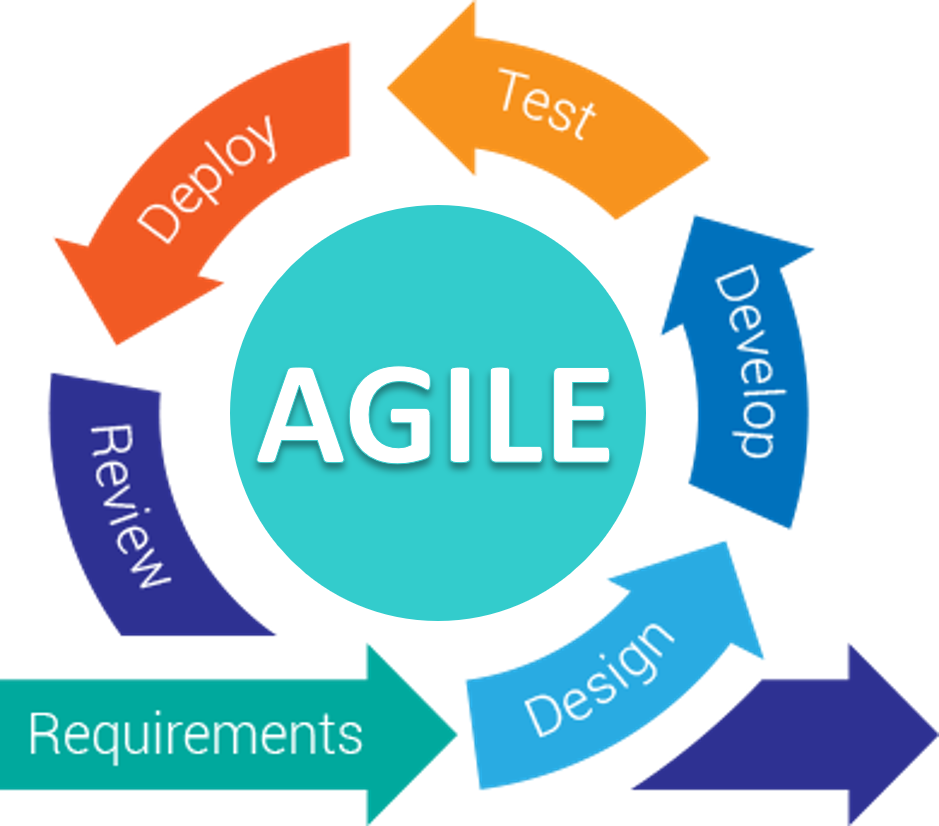
\includegraphics[width= 3in ]{agile.png}
%     \caption{Agile Model}
% \end{figure}
